%
% main.tex -- Paper zum Thema <clifford>
%
% (c) 2020 Hochschule Rapperswil
%
\chapter{Clifford Algebra\label{chapter:clifford}}
\lhead{Clifford Algebra}
\begin{refsection}
\chapterauthor{Thierry Schwaller, Marius Baumann}



GA [Geometric Algebra i.a.W. Clifford Algebra] provides a unified language for the whole of physics and for much of mathematics and its applications that is conceptually and computationally superior to alternative mathematical systems in many application domains.
\section{Vektoroperationen\label{clifford:section:Vektoroperationen}}
\rhead{Vektoroperationen}
\subsection{Vektordarstellung\label{clifford:section:Vektordarstellung}}
Vektoren können neben der üblichen Spaltendarstellung, auch als Linearkombination aus Basisvektoren
\begin{equation}
    \begin{split}
    \textbf{a} 
    &=
    \begin{pmatrix} 
    a_1 \\ a_2 \\ \vdots \\ a_n   
    \end{pmatrix} 
    =
    a_1 \begin{pmatrix}
    1 \\ 0 \\ \vdots \\ 0  
    \end{pmatrix} 
    + 
    a_2\begin{pmatrix} 
    0 \\ 1 \\ \vdots \\ 0  
    \end{pmatrix} + \dots 
    + 
    a_n\begin{pmatrix}
    0 \\ 0 \\ \vdots \\ 1  
    \end{pmatrix} \\\ 
    &= 
    a_1\textbf{e}_1 
    +
    a_2\textbf{e}_2
    + 
    \dots + a_n\textbf{e}_n
    = 
    \sum_{i=1}^{n} a_i \textbf{e}_i
    \qquad
    a_i \in \mathbb{R}
    , \textbf{e}_i \in \mathbb{R}^n
    \end{split}
\end{equation}
dargestellt werden.
Diese Basisvektoren werden so gewählt, dass sie orthonormal sind. 
Um die Darstellung zu vereinfachen werden sie durch $\textbf{e}_1 , \textbf{e}_2, \dots$ ersetzt.
\begin{beispiel}
Eine Linearkombination von Basisvektoren in $\mathbb{R}^4$ könnte wie folgt aussehen
    \begin{equation}
        \begin{pmatrix} 
        42 \\ 2 \\ 1291 \\ 4    
        \end{pmatrix} 
        = 
        42 \begin{pmatrix}
        1 \\ 0 \\ 0 \\ 0 
        \end{pmatrix} 
        +
        2 \begin{pmatrix} 
        0 \\ 1 \\ 0 \\ 0 
        \end{pmatrix}
        +
        1291 
        \begin{pmatrix} 
        0 \\ 0 \\ 1 \\ 0 
        \end{pmatrix} 
        +
        4 \begin{pmatrix} 
        0 \\ 0 \\ 0 \\ 1 
        \end{pmatrix} 
        = 
        42\textbf{e}_1
        + 
        2\textbf{e}_2
        + 
        1291\textbf{e}_3
        + 
        4\textbf{e}_4.
    \end{equation}
Dieses Beispiel ist für einen vier dimensionalen Vektor, dies kann selbstverständlich für beliebig viele Dimensionen nach demselben Schema erweitert werden.
\end{beispiel}

\subsection{Quadrat von Vektoren}
\subsubsection{Ziel der Multiplikation}
\index{Multiplikation}%
Was eine Addition von Vektoren bedeutet ist sehr intuitiv und auch leicht geometrisch darzustellen wie in Abbildung \ref{figure:addition}. Was allerdings das Produkt von Vektoren ergibt, mag anfänglich unintuitiv wirken.
\begin{figure}[tb]
	\centering
		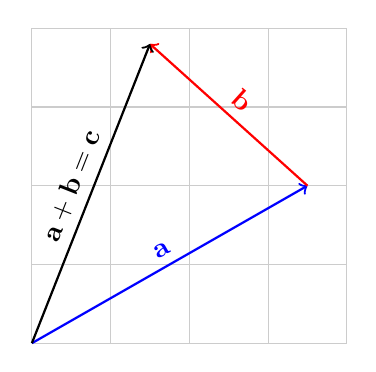
\begin{tikzpicture}
			\draw[thin,gray!40] (0,0) grid (4,4);
			\draw[blue,thick,->] (0,0)--(3.5,2) node[midway,above,sloped] {$\textbf{a}$};
			\draw[red,thick,->] (3.5,2)--(1.5,3.8) node[midway,above,sloped] {$\textbf{b}$};
			\draw[black,thick,->] (0,0)--(1.5,3.8)node[midway,above,sloped] {$\textbf{a} +\textbf{b} = \textbf{c} $};
		\end{tikzpicture}
		\caption{Addition von zwei Vektoren\label{figure:addition}}
\end{figure}
Was soll es schon heissen zwei Vektoren miteinander zu multiplizieren? 
Im Folgenden werden wir versuchen diese Operation ähnlich intuitiv darzustellen.

Um sinnvoll eine neue Operation zwischen zwei Elementen einer Algebra, in diesem Fall sind diese Elemente Vektoren, zu definieren, muss man überlegen, was das Ziel dieser Operation sein soll.
 
\begin{ziel}
	\label{clifford:ziel}
	Der Vektorraum der $n$-dimensionalen Vektoren soll zu einer Algebra so erweitert werden, dass das Quadrat von Vektoren durch die Länge des Vektors ausgedrückt werden kann.
\end{ziel}
Zusätzlich soll auch das Assoziativgesetz für die Multiplikation von Vektoren gelten, das heisst wir dürfen wie in
\index{Assoziativgesetz}%
\begin{equation*}
    \label{eq:assoziativ}
    \textbf{e}_i(\textbf{e}_j + \textbf{e}_k) 
    = 
    \textbf{e}_i\textbf{e}_j + \textbf{e}_i\textbf{e}_k
\end{equation*}
ausklammern.
Allerdings gilt das Kommutativgesetz leider oder, wie man sehen wird, zum Glück nur für skalare Elemente wie in
\index{Kommutativgesetz}%
\begin{equation}
    \label{eq:kommSkalar}
    a\textbf{e}_ib\textbf{e}_j 
    = 
    ab\textbf{e}_i\textbf{e}_j \qquad a,b \in \mathbb{R},
\end{equation}
aber nicht für Vektoren. Im Allgemeinen wird
\begin{equation}
    \label{eq:kommVector}
    \textbf{e}_i\textbf{e}_j 
    \neq 
    \textbf{e}_j\textbf{e}_i
\end{equation}
sein.
\subsubsection{Quadrieren eines Vektors}
\index{Quadrieren}%
Betrachten wir nun mit diesen Regeln das Quadrat eines Vektors.
Zuerst werden die Vektoren als Linearkombinationen geschrieben:
\begin{equation}
	    \textbf{a}^2 = 
		\biggl( 
		\sum_{i=1}^{n} a_i \textbf{e}_i 
		\biggr) 
		\biggl( 
		\sum_{i=1}^{n} a_i \textbf{e}_i 
		\biggr)
		\label{eq:quad_a_1}.
\end{equation}
Das Quadrat kann nun in zwei Summen 
\begin{equation}
	\textbf{a}^2 =
	\textcolor{red}{\sum_{i=1}^{n} a_i^2\textbf{e}_i^2} 
	+ 
	\textcolor{blue}{\sum_{\begin{subarray}{l}i,j=1\\i \neq j\end{subarray}}^n  a_ia_j\textbf{e}_i\textbf{e}_j } 
	\label{eq:quad_a_2}
\end{equation}
aufgeteilt werden, wobei die roten Summe die quadrierten Terme und die blaue Summe die Mischterme beinhaltet.
Wie zuvor in Ziel~\ref{clifford:ziel} definiert, ergibt das Quadrat eines Vektors dessen Länge
 Da die Basisvektoren orthonormiert sind, muss $\textbf{e}_i^2 = 1$ gelten:
\begin{equation}
	\textbf{a}^2 = \textcolor{red}{\sum_{i=1}^{n} a_i^2} + \textcolor{blue}{\sum_{\begin{subarray}{l}i,j=1\\i \neq j\end{subarray}}^n  a_ia_j\textbf{e}_i\textbf{e}_j}.
	\label{eq:quad_a_3}
\end{equation}
\begin{beispiel}
Das Quadrat des Vektor $\textbf{a}$ in $\mathbb{R}^2$ ist
\begin{align*}
    \textbf{a}^2 
    &= (a_1\textbf{e}_1+a_2\textbf{e}_2)(a_1\textbf{e}_1+a_2\textbf{e}_2) \\
    &= \textcolor{red}{a_1^2\textbf{e}_1^2 + a_2^2\textbf{e}_2^2} 
    + \textcolor{blue}{a_1\textbf{e}_1a_2\textbf{e}_2 + a_2\textbf{e}_2a_1\textbf{e}_2}   \\
    & = \textcolor{red}{a_1^2 + a_2^2} + \textcolor{blue}{a_1b\textbf{e}_1a_2\textbf{e}_2 + a_2\textbf{e}_2a_1\textbf{e}_2}.
\qedhere
\end{align*}
\end{beispiel}

Der rote Teil von \eqref{eq:quad_a_3} ist nun bereits die Länge im Quadrat, also das zuvor definierte Ziel der Multiplikation.
Daraus lässt sich schliessen, dass der restliche Teil dieser Gleichung
\begin{equation}
    \label{eq:Mischterme_Null}
    \sum_{\begin{subarray}{l}i,j=1\\i \neq j\end{subarray}}^n  a_ia_j\textbf{e}_i\textbf{e}_j  = \textcolor{blue}{a_1a_2(\textbf{e}_1\textbf{e}_2 + \textbf{e}_2\textbf{e}_1)} + a_1a_3(\textbf{e}_1\textbf{e}_3 + \textbf{e}_3\textbf{e}_1) + \dots =  0.
\end{equation}
 ergeben muss.
 Aus dieser Erkenntnis können weitere Eigenschaften für die Multiplikation hergeleitet werden.
 
Da dies für beliebige $a_i$ gelten muss, werden alle Terme bis auf $a_1$ und $a_2$ gleich null gesetzt.
Somit fallen alle Terme bis auf den blauen weg.
Wird dies weiter vereinfacht, ergibt sich
\begin{equation*}
\begin{aligned}
    a_1a_2(\textbf{e}_1\textbf{e}_2 + \textbf{e}_2\textbf{e}_1) &= 0 \\
    a_1a_2\textbf{e}_1\textbf{e}_2 &= -a_1a_2\textbf{e}_2\textbf{e}_1 \\
    \textbf{e}_1\textbf{e}_2 &= -\textbf{e}_2\textbf{e}_1.
\end{aligned}
\end{equation*}
\begin{satz}
  Die Multiplikation von orthogonalen Vektoren ist antikommutativ:
    \begin{equation*}
        \mathbf{e}_i\mathbf{e}_j = -\mathbf{e}_j\mathbf{e}_i \quad \textrm{für} \quad \mathbf{e}_i \perp \mathbf{e}_j.
    \end{equation*}
\end{satz}
Dieses Wissen reicht nun bereits, um alle Produkte der Basisvektoren zu berechnen, was in Tabelle \ref{tab:multip_vec} gemacht wurde.
\begin{table}
\begin{center}
\begin{tabular}{ |c|ccccc| } 
 \hline
  & $\textbf{e}_1$ & $\textbf{e}_2$ & $\dots$ & $\textbf{e}_{n-1}$ & $\textbf{e}_{n}$ \\
  \hline
 $\textbf{e}_1$ & 1 & $\textbf{e}_1\textbf{e}_2$ & $\dots$ & $\textbf{e}_1\textbf{e}_{n-1}$ & $\textbf{e}_1\textbf{e}_{n}$ \\
 $\textbf{e}_2$ & $-\textbf{e}_1\textbf{e}_2$ & 1 & $\dots$ & $\textbf{e}_2\textbf{e}_{n-1}$ & $\textbf{e}_2\textbf{e}_{n}$ \\
 $\vdots$ & $\vdots$ & $\vdots$ & $\ddots$ & $\vdots$ & $\vdots$ \\
 $\textbf{e}_{n-1}$ & $-\textbf{e}_1\textbf{e}_{n-1}$ & $-\textbf{e}_2\textbf{e}_{n-1}$  & $\dots$ & $1$ & $\textbf{e}_{n-1}\textbf{e}_{n}$ \\
 $\textbf{e}_{n}$ & $-\textbf{e}_1\textbf{e}_{n}$ & $-\textbf{e}_2\textbf{e}_{n}$  & $\dots$ & $-\textbf{e}_{n-1}\textbf{e}_{n}$ & 1 \\
 \hline
\end{tabular}
\end{center}
\caption{Multiplikationstabelle für Vektoren}
\label{tab:multip_vec}
\end{table}

\subsection{Multiplikation von Vektoren}
Was geschieht nun wenn zwei beliebige Vektoren, $u$ und $v$
\begin{equation}
    \textbf{u} = 
    \sum_{i=1}^{n} u_i \textbf{e}_i 
    \qquad 
    \textbf{v} = \sum_{i=1}^{n} v_i \textbf{e}_i
\end{equation}
 miteinander multipliziert werden? 
 
 Wieder werden die Vektoren zuerst als Linearkombinationen darstellen und danach in zwei Summen aufgeteilt, eine Summe mit quadrierten Termen und eine Summe mit Mischtermen
\begin{equation}
    \begin{split}
        \textbf{u}\textbf{v} 
        =
        \left ( 
        \sum_{i=1}^{n} u_i \textbf{e}_i
        \right ) 
        \left ( 
        \sum_{i=1}^{n} v_i \textbf{e}_i
        \right) 
        = 
        \sum_{i=1}^n u_iv_i\underbrace{\textbf{e}_i^2}_{1} 
        + \sum_{\begin{subarray}{l}i,j=1\\i \neq j\end{subarray}}^n  u_iv_j\textbf{e}_i\textbf{e}_j,
    \end{split}
\end{equation}
wobei die Summe der quadrierten Termen bereits bekannt vorkommen könnte, es ist nämlich das Skalarprodukt von $u$ und $v$. Die Summe der Mischterme bilden etwas neues, dass wir das äussere Produkt von $u$ und $v$ nennen.
\begin{beispiel}
    Multiplikation von Vektoren in $\mathbb{R}^2$
\begin{equation}
    \begin{split}
        \textbf{u}\textbf{v} 
        &= 
        (u_1\textbf{e}_1 + u_2\textbf{e}_2)(v_1\textbf{e}_1 + v_2\textbf{e}_2) 
        = 
        u_1v_1\textbf{e}_1^2
        + 
        u_2v_2\textbf{e}_2^2 
        + 
        u_1v_2\textbf{e}_1\textbf{e}_2 
        +  
        u_2v_1\underbrace{\textbf{e}_2\textbf{e}_1}_{-\textbf{e}_1\textbf{e}_2}
        \\\ 
        &=  
        \underbrace{(u_1v_1 + u_2v_2)}_{\text{Skalarprodukt}} 
        + 
        \underbrace{(u_1v_2 - u_2v_1)\textbf{e}_1\textbf{e}_2}_{\text{Äusseres Produkt}}
    \end{split}
\end{equation}
\end{beispiel}
\subsubsection{Äusseres Produkt}
Das äussere Produkt von zwei Vektoren wird mit einem $\wedge$ dargestellt
\begin{equation}
    \textbf{u}\wedge \textbf{v} 
    = 
    \sum_{\begin{subarray}{l}i,j=1\\i \neq j\end{subarray}}^n  u_iv_j\textbf{e}_i\textbf{e}_j 
\end{equation}
\begin{beispiel}
Das äusseres Produkt von zwei Vektoren in $\mathbb{R}^3$ ist
\begin{equation}
	\begin{split}
		u \wedge v 
		&= 
		u_1v_2\textbf{e}_1\textbf{e}_2 
		+ 
		u_1v_3\textbf{e}_1\textbf{e}_3 
		+ 
		u_2v_2\textbf{e}_2\textbf{e}_3 
		+ 
		u_2v_1\textbf{e}_2\textbf{e}_1 
		+ 
		u_3v_1\textbf{e}_3\textbf{e}_1 
		+
		u_3v_2\textbf{e}_3\textbf{e}_2 \\\ 
		&= 
		(u_1v_2 - u_2v_1)\textbf{e}_1\textbf{e}_2 
		+ 
		(u_1v_3 - v_3u_1)\textbf{e}_1\textbf{e}_3 
		+ 
		(u_2v_3 - u_3v_2)\textbf{e}_2\textbf{e}_3.
	\end{split}
\end{equation}
\end{beispiel}

Im letzten Schritt des Beispiels wurden nun, mit Hilfe der antikommutativität des Produkts, die Vektorprodukte, welche die gleichen Einheitsvektoren beinhalten, zusammengefasst. Dieses Vorgehen kann man auch allgemein anwenden, wie in den Gleichungen \eqref{eq:u_wedge_v}-\eqref{eq:u_wedge_v_5} hergeleitet. Die Summe,
\begin{align}
        \textbf{u}\wedge \textbf{v}
        &= 
        \sum_{\begin{subarray}{l}i,j=1\\i \neq j\end{subarray}}^n  
        u_iv_j\textbf{e}_i\textbf{e}_j,
        \label{eq:u_wedge_v}
        \intertext{wird in zwei verschiedene Summen aufgeteilt. 
        	Wobei die linke Summe jeweils den Basisvektor mit dem höheren Index an erster Stelle und die rechte Summe diesen jeweils an zweiter Stelle hat}
        \label{eq:u_wedge_v_1}
        &= 
        \sum_{\begin{subarray}{l}i,j=1\\i < j\end{subarray}}^n u_iv_j\textbf{e}_i\textbf{e}_j 
        + 
        \sum_{\begin{subarray}{l}i,j=1\\j < i\end{subarray}}^n u_iv_j\textbf{e}_i\textbf{e}_j. 
        \intertext{Nun werden die Indexe der zweiten Summe vertauscht}
        \label{eq:u_wedge_v_2}
        &= 
        \sum_{\begin{subarray}{l}i,j=1\\i < j\end{subarray}}^n u_iv_j\textbf{e}_i\textbf{e}_j 
        + 
        \sum_{\begin{subarray}{l}i,j=1\\i < j\end{subarray}}^n u_jv_i\textbf{e}_j\textbf{e}_i,
       	\intertext{und diese wird nun mit Hilfe der Antikommutativität umgeformt zu}
        &= 
        \sum_{\begin{subarray}{l}i,j=1\\i < j\end{subarray}}^n u_iv_j\textbf{e}_i\textbf{e}_j 
        - 
        \sum_{\begin{subarray}{l}i,j=1\\i < j\end{subarray}}^n u_jv_i\textbf{e}_i\textbf{e}_j.
        \intertext{Nun können die zwei Summen wieder zusammengefasst werden}
        \label{eq:u_wedge_v_4}
        &= 
        \sum_{\begin{subarray}{l}i,j=1\\i < j\end{subarray}}^n (u_iv_j -u_jv_i)\textbf{e}_i\textbf{e}_j.
        \intertext{Der Term in der Summe könnte einem bereits bekannt vorkommen, es ist nämlich die Determinante einer Matrix mit $u$ und $v$ als ihre Spalten}
        &= 
        \label{eq:u_wedge_v_5}
        \sum_{\begin{subarray}{l}i,j=1\\i < j\end{subarray}}^n \begin{vmatrix} 
        u_i & v_i \\
        u_j & v_j
    \end{vmatrix}\textbf{e}_i\textbf{e}_j.
\end{align}
Die Determinante einer Matrix beschreibt die Fläche, welche von den Spaltenvektoren aufgespannt wird, wie in Abbildung \ref{figure:det} dargestellt.
\begin{figure}[htb]
	\centering
	\begin{minipage}[t]{.45\linewidth}
		\centering
		\begin{tikzpicture}
			\draw[thin,gray!40] (0,0) grid (4,4);
			\draw[<->] (0,0)--(4,0) ;
			\draw[<->] (0,0)--(0,4) ;
			\draw[line width=0,fill=gray!40] (0,0)--(3,1)--(4,3)--(1,2);
			\draw[line width=2pt,blue,-stealth](0,0)--(3,1) node[anchor=north
			west]{$\boldsymbol{u}$};
			\draw[line width=2pt,red,-stealth](0,0)--(1,2) node[anchor=south east]{$\boldsymbol{v}$};
			\draw[black] (2,1.5)--(1.8,3.2) node[anchor = south]{$\begin{vmatrix} 
					u_i & v_i \\
					u_j & v_j
				\end{vmatrix} = u_iv_j - v_iu_j$};
		\end{tikzpicture}
		\caption{Geometrische Interpretation der Determinante einer $2 \times 2$ Matrix\label{figure:det}}
	\end{minipage}%
	\hfill%
	\begin{minipage}[t]{.45\linewidth}
		\centering
		\begin{tikzpicture} 
			\draw[thin,gray!40] (0,0) grid (4,4);
			\draw[<->] (0,0)--(4,0) node[right]{$x$};
			\draw[<->] (0,0)--(0,4) node[above]{$y$};
			\draw[line width=0,fill=gray!40] (0,0)--(3,1)--(4,3)--(1,2);
			\draw[line width=2pt,blue,-stealth](0,0)--(3,1) node[anchor=north
			west]{$\boldsymbol{u}$};
			\draw[line width=2pt,red,-stealth](0,0)--(1,2) node[anchor=south east]{$\boldsymbol{v}$};
			\draw[->] (2.15,1.5) arc (0:310:0.3);
			\draw[black] (2,1.5)--(2.5,3.2) node[anchor = south]{$u\wedge v = \begin{vmatrix} 
					u_i & v_i \\
					u_j & v_j
				\end{vmatrix} e_1e_2 = (u_iv_j - v_iu_j)\textbf{e}_1\textbf{e}_2$};
		\end{tikzpicture}
		\caption{Geometrische Interpretation des äusseren Produktes \label{figure:wedge}}
	\end{minipage}
\end{figure}
Das äussere Produkt besteht nun also aus der Summe 
    \(\sum_{\begin{subarray}{l}i,j=1\\i < j\end{subarray}}^n\)
    von Flächen 
    \(\begin{vmatrix} 
    	u_i & v_i \\
    	u_j & v_j
    \end{vmatrix}\)
, welche in $\textbf{e}_i\textbf{e}_j$ aufgespannt sind, wie man in \ref{eq:u_wedge_v_5} sieht. 
Dieses Produkt $\textbf{e}_i\textbf{e}_j$ der Basisvektoren interpretiert man als Umlaufrichtung.
Wobei die gebildete Fläche in Richtung des ersten Vektors umschritten wird. 
Dies ist in Abbildung \ref{figure:wedge} dargestellt, wobei bei diesem Beispiel die Umlaufrichtung im Gegenuhrzeigersinn ist, da die Fläche in Richtung u umschritten wird. 
Diese Fläche mit einer Richtung nennt man in der geometrischen Algebra einen Bivektor, da er eine Art zwei dimensionaler Vektor ist. 

\subsection{Geometrisches Produkt}
Die Multiplikation von zwei Vektoren nennt man in der Clifford Algebra das geometrische Produkt, dieses können wir nun als Summe aus dem Skalar- und dem äusseren Produkt darstellen
\begin{equation}
    \textbf{u}\textbf{v} = \textbf{u}\cdot \textbf{v} + \textbf{u} \wedge \textbf{v}.
\end{equation}
Dieses Additionszeichen zwischen diesen zwei Produkten mag vielleicht ein wenig eigenartig wirken, da uns das Skalarprodukt ein Skalar und das äussere Produkt einen Bivektor zurück gibt. Was bedeutet es nun also diese beiden Elemente zu addieren?
Man kann sich die Addition wie bei den komplexen Zahlen vorstellen, wobei die imaginäre Einheit auch nicht explizit zu dem reelen Teil addiert werden kann, sondern die zwei Teile zusammen ein Objekt, eine komplexe Zahl bilden. 
Dieses Objekt, also die Summe von verschiedenen Elemente der Clifford Algebra, wird Multivektor genannt.
\begin{definition}
Ein Multivektor besteht aus den verschiedenen Bauteilen, wie zum Beispiel Vektoren, Bivektoren oder Trivektoren (Volumen mit einer Richtung), der Clifford Algebra.
\begin{equation}
    M = \sum \left ( \prod a_i\textbf{e}_j \right)
\end{equation}
\end{definition}
Besteht eine Clifford Algebra aus n Basisvektoren so hat sie n Dimensionen, dies wird nicht wie in der linearen Algebra mit $\mathbb{R}^n$ sondern mit $\mathbb{G}^n$ beschrieben. 
\begin{beispiel}
Allgemeiner Multivektor in $\mathbb{G}^3$
\begin{equation}
    M = a 
    + 
    \underbrace{b\textbf{e}_1 + c\textbf{e}_2 + d\textbf{e}_3}_{\text{Vektorteil}} 
    +
    \underbrace{f\textbf{e}_1\textbf{e}_2 + g\textbf{e}_1\textbf{e}_3 + h\textbf{e}_2\textbf{e}_3 }_{\text{Bivektorteil}} 
    +   
    \underbrace{k\textbf{e}_1\textbf{e}_2\textbf{e}_3}_{\text{Trivektorteil}}
\end{equation}
\end{beispiel}
\begin{definition}
Um das Produkt von Basisvektoren in Zukunft darzustellen wird folgende Notation definiert
    \begin{equation}
        e_ie_j = e_{ij}
    \end{equation}
\end{definition}
Nun da das geometrische Produkt vollständig definiert wurde können Multiplikationstabellen für verschiedene Dimensionen $\mathbb{G}^n$ erstellt werden. In \ref{tab:multip} ist dies für  $\mathbb{G}^3$ gemacht.
\begin{table}
    \caption{Multiplikationstabelle für $\mathbb{G^3}$}
    \label{tab:multip}
    \begin{center}
    \begin{tabular}{ |c|c|c|c|c|c|c|c| } 
     \hline
     1 & $\textbf{e}_1$ & $\textbf{e}_2$ &$\textbf{e}_3$ & $\textbf{e}_{12}$ & $\textbf{e}_{13}$ & $\textbf{e}_{23}$ & $\textbf{e}_{123}$\\
     \hline
     $\textbf{e}_1$ & 1 & $\textbf{e}_{12}$ & $\textbf{e}_{12}$ & $\textbf{e}_2$ & $\textbf{e}_3$ & $\textbf{e}_{123}$ & $\textbf{e}_{23}$\\
     \hline
     $\textbf{e}_2$ & $-\textbf{e}_{12}$ & 1 & $\textbf{e}_{23}$ & $-\textbf{e}_1$ & $-\textbf{e}_{123}$ & $\textbf{e}_3$ & $-\textbf{e}_{13}$\\
     \hline
     $\textbf{e}_3$ & $-\textbf{e}_{13}$ & $-\textbf{e}_{23}$ & 1 & $\textbf{e}_{123}$ & $-\textbf{e}_1$ & $-\textbf{e}_2$ & $\textbf{e}_{12}$\\
     \hline
     $\textbf{e}_{12}$ & -$\textbf{e}_2$ & $\textbf{e}_1$& $\textbf{e}_{123}$ & -1 & $-\textbf{e}_{23}$ & $\textbf{e}_{13}$ &  $-\textbf{e}_{3}$\\
     \hline
     $\textbf{e}_{13}$ & $-\textbf{e}_{3}$ & $-\textbf{e}_{123}$ & $\textbf{e}_{1}$ & $\textbf{e}_{23}$ & -1 & $-\textbf{e}_{12}$ &  $\textbf{e}_{2}$\\
     \hline
     $\textbf{e}_{23}$ &  $\textbf{e}_{123}$ & $-\textbf{e}_{3}$ & $\textbf{e}_{2}$ & $-\textbf{e}_{13}$ & $\textbf{e}_{12}$ & -1 & $-\textbf{e}_{1}$ \\
     \hline
     $\textbf{e}_{123}$ & $\textbf{e}_{23}$ & $-\textbf{e}_{13}$ & $\textbf{e}_{12}$ & $-\textbf{e}_{3}$& $\textbf{e}_{2}$ & $-\textbf{e}_{1}$ & -1 \\
     \hline
    \end{tabular}
    \end{center}
\end{table}

\subsection{Polare Darstellung des geometrischen Produktes}
Beide Teile des geometrischen Produktes lassen sich durch trigonometrische Terme beschreiben. Das Skalarprodukt kann als 
\begin{equation}
    \textbf{u}\cdot \textbf{v} = |\textbf{u}||\textbf{v}|\cos{\alpha}
\end{equation}
beschrieben werden. Wobei $\alpha$ der Winkel zwischen $\textbf{u}$ und $\textbf{v}$ ist.

Beim äusseren Produkt wurde bereits erwähnt, dass es aus dem Produkt der Fläche des von den zwei Vektoren aufgespannten Parallelogram und einer Umlaufrichtung beschrieben wird. Die Fläche eines Parallelograms lässt sich auch mit einen Sinus Term
\begin{equation}
    \textbf{u} \wedge \textbf{v}
    = 
    \sum_{i<j}
    \begin{vmatrix} 
        u_i & v_i \\
        u_j & v_j
    \end{vmatrix}\textbf{e}_i\textbf{e}_j  
    = 
    \underbrace{|u||v|\sin{\alpha}}_{\text{Fläche}}\textbf{b}_1\textbf{b}_2
\end{equation}
beschreiben.
Die Fläche des Parallelogramms liegt dabei auf der von $\textbf{b}_1$ und $\textbf{b}_2$ aufgespannten Ebene.

Nun kann man diese Terme wieder zum geometrischen Produkt
\begin{equation}
    \textbf{u}\textbf{v}
    = 
    |\textbf{u}||\textbf{v}|\cos{(\alpha)} 
    + 
    |\textbf{u}||\textbf{v}|\sin{(\alpha)} \textbf{b}_1\textbf{b}_2
    = 
    |\textbf{u}||\textbf{v}|(\cos{(\alpha)} + \sin{(\alpha)}\textbf{b}_1\textbf{b}_2)
\end{equation}
vereinen.
Daraus kann geschlussfolgert werden, dass
\begin{equation}
	\textbf{u} \textbf{v}=-\textbf{v}\textbf{u} \quad \textrm{für} \quad \textbf{u}\perp \textbf{v} 
	\label{uperpv}
\end{equation}
und
\begin{equation}
	\textbf{u} \textbf{v}=\textbf{v}\textbf{u} \quad \textrm{für} \quad \textbf{u} \parallel \textbf{v} 
	\label{uparallelv}
\end{equation}
gilt.
%
% einleitung.tex -- Beispiel-File für die Einleitung
%
% (c) 2020 Prof Dr Andreas Müller, Hochschule Rapperswil
%
\section{Pauli-Matrizen}
\rhead{Pauli-Matrizen}

Was ist der beste Weg um einen Computeralgorithmus für die Rechenoperationen in der Clifford-Algebra zu erstellen? Man könnte versuchen einen textuellen Rechner zu implementieren der für die Elemente $\mathbf{e}_i$ hartkodierte Vereinfachungen ausführt 
\begin{beispiel}
	Der Algorithmus weiss, dass er $a\mathbf{e}_1\cdot b\mathbf{e}_1$ zu $ab\cdot1$ vereinfachen kann
	\begin{align}
		3\mathbf{e}_1 \cdot 2\mathbf{e}_1 + 3\mathbf{e}_2 \Rightarrow 6 + 3\mathbf{e}_2
	\end{align}
\end{beispiel}
Dies ist aber sehr ineffizient. Die Pauli-Matrizen bilden eine elegante und schnellere Alternative, welche für die dreidimensionale Clifford-Algebra verwendet werden können und alle Operationen aus der Clifford-Algebra gleich wie die Matrixoperationen ausführen lassen.
\begin{definition} \label{def:defPauli}
	Die Matrizen
	\begin{align}
		\mathbf{e}_0 = E = 
		\begin{pmatrix}
			1 & 0 \\
			0 & 1
		\end{pmatrix}\quad
		\mathbf{e}_1 =
		\begin{pmatrix}
			0 & 1 \\
			1 & 0
		\end{pmatrix}\quad
		\mathbf{e}_2 =
		\begin{pmatrix}
			0 & -j \\
			j & 0
		\end{pmatrix}\quad
		\mathbf{e}_3 =
		\begin{pmatrix}
			1 & 0 \\
			0 & -1
		\end{pmatrix}\quad	
	\end{align}
	heissen Pauli-Matrizen ($\mathbf{e}_0$ = Skalare)
\end{definition}
Die Matrix-Multiplikationen der Pauli-Matrizen führt auf die gleichen algebraischen Relationen, wie die Multiplikation der Elemente $\mathbf{e}_0, \mathbf{e}_1, \mathbf{e}_2, \mathbf{e}_3$. So lassen sich auch die restlichen Elemente der Clifford-Algebra herleiten.
\begin{definition} \label{def:defPauli2}
	Die Bivektoren und Trivektoren hergeleitet durch die Pauli-Matrizen
	\begin{align}
		\mathbf{e}_{12} =  
		\begin{pmatrix}
			j & 0 \\
			0 & -j
		\end{pmatrix}\quad
		\mathbf{e}_{23} =
		\begin{pmatrix}
			0 & j \\
			j & 0
		\end{pmatrix}\quad
		\mathbf{e}_{31} =
		\begin{pmatrix}
			0 & 1 \\
			-1 & 0
		\end{pmatrix}\quad
		\mathbf{e}_{123} =
		\begin{pmatrix}
			j & 0 \\
			0 & j
		\end{pmatrix}\quad	
	\end{align}
\end{definition}
Dabei ist wichtig, dass sich die Matrizen gleich verhalten, wie es die Clifford-Algebra für die Basiselemente definiert hat.
\begin{align}
	\mathbf{e}_1^2 &=
	\begin{pmatrix}
		0 & 1 \\
		1 & 0
	\end{pmatrix}^2 = 
	\begin{pmatrix}
		1 & 0 \\
		0 & 1
	\end{pmatrix}= \mathbf{e}_0 \\
	\mathbf{e}_{12}^2 &=
	\begin{pmatrix}
		j & 0 \\
		0 & -j
	\end{pmatrix}^2 = 
	\begin{pmatrix}
		-1 & 0 \\
		0 & -1
	\end{pmatrix} = -\mathbf{e}_0 
\end{align}
Man kann bei den Definitionen \ref{def:defPauli} und \ref{def:defPauli2} sehen, dass alle Matrizen linear unabhängig voneinander sind. Das bedeutet, dass wenn man die Matrizen der Basiselemente normal addiert und zu einer Matrix zusammenfasst, kann man anschliessend die einzelnen Anteile der Basiselemente wieder herausgelesen.
\begin{definition}
	Multivektor mit Pauli-Matrizen
	\begin{align}
		M &= a_0\mathbf{e}_0 + a_1\mathbf{e}_1 + a_2\mathbf{e}_3 + a_{12}\mathbf{e}_{12} + a_{23}\mathbf{e}_{23} + a_{31}\mathbf{e}_{31} + a_{123}\mathbf{e}_{123}\\
		M &=
		\begin{pmatrix}
			(a_0+a_3) + (a_{12}+a_{123})j & (a_1+a_{31})+(-a_2+a_{23})j \\
			(a_1-a_{31})+(a_2+a_{23})j & (a_0-a_3)+(-a_{12}+a_{123})j
		\end{pmatrix}  
	\end{align}
\end{definition}
Die Anteile treten zudem immer paarweise auf und können somit immer je durch zwei Gleichungen bestimmt werden.
\begin{beispiel}
	Bestimmung der Anteile der Basiselemente
	\begin{align}
		M &= 
		\begin{pmatrix}
			1 & 0 \\
			0 & 0
		\end{pmatrix}\\
		&\Rightarrow a_0 + a_3 = 1 \enspace\land\enspace a_0 - a_3 = 0\\
		&\Rightarrow a_0 = \dfrac{1}{2} \enspace\land\enspace a_3 = \dfrac{1}{2}\\
		M &= \dfrac{1}{2} \mathbf{e}_0+ \dfrac{1}{2} \mathbf{e}_3
	\end{align}
\end{beispiel}
Die Clifford-Algebra bei der Darstellung durch Matrizen kein Ausnahmefall. Es lässt sich theoretisch jede algebraische Struktur durch Matrizen darstellen.
%
% teil1.tex -- Beispiel-File für das Paper
%
% (c) 2020 Prof Dr Andreas Müller, Hochschule Rapperswil
%
\section{Spiegelung}
\rhead{Spiegelung}

Die Spiegelung ist eine grundlegende, geometrische Operation, aus welcher man weitere Operationen, wie beispielsweise die später beschriebene Rotation, ableiten kann. Da die geometrische Algebra für geometrische Anwendungen ausgelegt ist, sollte die Spiegelung auch eine einfache, praktische Formulierung besitzen.
\begin{figure}
	\centering
	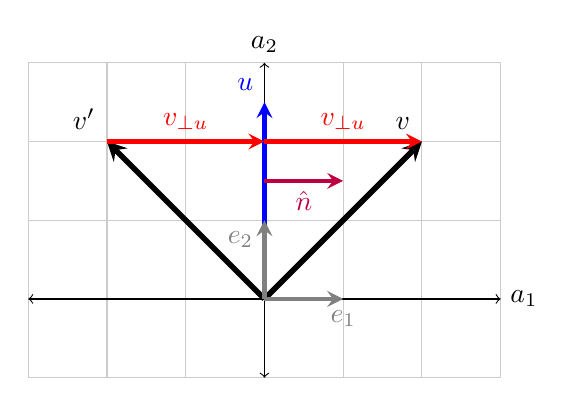
\begin{tikzpicture}
		\draw[thin,gray!40] (-3,-1) grid (3,3);
		\draw[<->] (-3,0)--(3,0) node[right]{$a_1$};
		\draw[<->] (0,-1)--(0,3) node[above]{$a_2$};
		\draw[line width=2pt,black,-stealth](0,0)--(2,2) node[anchor=south east]{$\boldsymbol{v}$};
		\draw[line width=1.5pt,blue,-stealth](0,0)--(0,2.5) node[anchor=south east]{$\boldsymbol{u}$};
		\draw[line width=2pt,black,-stealth](0,0)--(-2,2) node[anchor=south east]{$\boldsymbol{v'}$};
		\draw[line width=1.5pt,gray,-stealth](0,0)--(1,0) node[anchor=north]{$\boldsymbol{e_1}$};
		\draw[line width=1.5pt,gray,-stealth](0,0)--(0,1) node[anchor=north east]{$\boldsymbol{e_2}$};
		\draw[line width=1.5pt,red,-stealth](0,2)--(2,2) node[xshift=-1cm, yshift=
		0.25cm]{$\boldsymbol{v_{\perp u}}$};
		\draw[line width=1.5pt,red,-stealth](-2,2)--(0,2) node[xshift=-1cm, yshift=
		0.25cm]{$\boldsymbol{v_{\perp u}}$};
		\draw[line width=1.5pt,purple,-stealth](0,1.5)--(1,1.5) node[xshift=-0.5cm, yshift=-0.25cm]{$\boldsymbol{\hat{n}}$};
	\end{tikzpicture}
	\caption{Spiegelung des Vektors \textbf{v} an Spiegelachse bzw. Vektor \textbf{u}}
	\label{BildSpiegelung}
\end{figure}

\subsection{Linearen Algebra}
Aus der linearen Algebra ist bekannt, dass man eine Spiegelung an einer Ebene wie folgt beschreiben kann.
\begin{definition}
	Die Spiegelungsgleichung in der linearen Algebra mit dem Normalenvektor $\mathbf{\hat{n}}$ zur Spiegelebene ist
	\begin{equation} \label{RefLinAlg}
		\mathbf{v^{'}} = \mathbf{v} - 2 \cdot \mathbf{v_{\parallel \hat{n}}} = \mathbf{v} - 2 \cdot \mathbf{v_{\perp u}}.
	\end{equation}
\end{definition}
Per Definition sind $\mathbf{v_{\parallel \hat{n}}} = \mathbf{v_{\perp u}}$, aber in der geometrischen Algebra verwenden wir bevorzugter weise in den Formeln Vektoren, welche eine Spiegelung an einer Hyperebene beschreiben. Im zweidimensionalen repräsentiert der Vektor $\mathbf{v^{'}}$ also eine Spiegelung vom Vektor $\mathbf{v}$ an einer Gerade und im dreidimensionalen eine Spiegelung an einer Ebene.
Es scheint für diese Formel \eqref{RefLinAlg} aber umständlich zu sein, weitere Spiegelungen mit weiteren Spiegelebenen anzufügen. Man kann diese Abbildung aber auch als Matrix schreiben. Sei $\mathbf{\hat{n}}$ ein Normalenvektor auf die Spiegelungs-Achse bzw. -Ebene, also $\mathbf{\hat{n}}\perp \mathbf{u}$, und sei ausserdem normiert $|\mathbf{\hat{n}}| = 1$, dann kann man die Spiegelung durch die Matrix
\begin{align}
	S = E - 2\dfrac{1}{|\mathbf{n}|^2}\mathbf{nn}^t
\end{align}
beschrieben werden. In der zweiten und dritten Dimension ergibt die Berechnung
\begin{align} \label{Spiegelmatrizen}
	S_2 = \begin{pmatrix}
		1-2n_1^2 & -2n_1n_2 \\
		-2n_1n_2 & 1-2n_2^2
	\end{pmatrix}\enspace\text{und}\enspace
	S_3 = \begin{pmatrix}
		1-2n_1^2 & -2n_1n_2 & -2n_1n_3\\
		-2n_1n_2 & 1-2n_2^2 & -2n_2n_3\\
		-2n_1n_3 & -2n_2n_3 & 1-2n_3^2\\
	\end{pmatrix}.
\end{align}
Diese Spiegelmatrizen gehören der orthogonalen Matrizengruppe $S_n\in \text{O}(n)$ an. Die Matrizengruppe $\text{O}(n)$ haben die Eigenschaft $S_n^t S_n = E$, was bedeutet, dass die Länge und Winkel bei der Abbildung beibehalten bleiben. Zusätzlich sind die Spiegelmatrizen symmetrisch, es gilt $S_n^t = S_n$. Somit liefert zweimal dieselbe Spiegelung wieder die identische Abbildung, wie man aus
\begin{align}
	S_n^t S_n = S_n^2 = E
\end{align}
schliessen kann.

\subsection{Geometrische Algebra}
Um die folgenden Formeln zu verstehen, definieren wir zuerst die Inverse eines Vektors, welche in dieser Form nicht in der linearen Algebra nicht existiert.
\begin{definition}
	Die Inverse eines Vektors wird definiert als
	\begin{align} \label{InverseGA}
		\mathbf{u}^{-1} = \dfrac{\mathbf{u}}{|\mathbf{u}|^2}. 
	\end{align}
\end{definition}
Diese Definition ist sinnvoll, da wegen $\mathbf{u}^2 = |\mathbf{u}|^2$ folgt
\begin{align}
	\mathbf{uu}^{-1} = \mathbf{u} \frac{\mathbf{u}}{|\mathbf{u}|^2} = \frac{\mathbf{u}^2}{|\mathbf{u}|^2} = \frac{|\mathbf{u}|^2}{|\mathbf{u}|^2} = 1.
\end{align}
Der Vektor $\mathbf{u}^{-1}$ in \eqref{InverseGA} ist also tatsächlich das inverse Element im Sinne des Produktes in der geometrischen Algebra.

Die geometrische Algebra leitet aus der obigen Formel \eqref{RefLinAlg} für eine Spiegelung eine einfache und intuitive Form her, welche auch für weitere Operationen erweitert werden kann.
\begin{definition}
	Die Spiegelungsgleichung in der geometrischen Algebra mit der Spiegelachse $\mathbf{u}$ ist definiert als
	\begin{align}\label{RefGA}
		\mathbf{v}' = \mathbf{uvu}^{-1}
	\end{align}
\end{definition}
Verwendet man für $\mathbf{u}$ nur einen Einheitsvektor $\mathbf{\hat{u}}$, welcher die Länge 1 besitzt, wird die Gleichung zu
\begin{align}
	\mathbf{v'} = \mathbf{\hat{u}v\hat{u}}
\end{align}
vereinfacht. Im Gegensatz zu den Abbildungen in der linearen Algebra, welche in jeder anderen Dimension, durch andere Matrizen \eqref{Spiegelmatrizen} beschrieben werden müssen, ist es in der geometrischen Algebra immer der gleiche Vorgehensweise. Zudem ist diese kompakte Schreibweise in der linearen Algebra nicht möglich, da bis auf das Vektorprodukt in der dritten Dimension keine Multiplikation von Vektoren definiert ist. 
%
% teil2.tex -- Beispiel-File für teil2 
%
% (c) 2020 Prof Dr Andreas Müller, Hochschule Rapperswil
%
\section{Rotation}
\rhead{Rotation}

Eine Rotation kann man aus zwei, aufeinanderfolgende Spiegelung bilden. Das war für mich zuerst eine verwirrende Aussage, da man aus den vorherig gezeigten Formeln annehmen könnte, dass die Spiegelung schon für eine Drehung ausreicht. Obwohl sich die Längen, Winkel und Volumen sich bei einer Spiegelung, wie bei einer Rotation, nicht ändert, sind sie doch verschieden, da die Orientierung bei der Spiegelung invertiert wird. Stellt man sich beispielsweise ein Objekt im Dreidimensionalen vor und spiegelt dieses an einer Fläche, dann ist es unmöglich nur durch eine Rotation (egal an welchem Punkt) das ursprüngliche Objekt deckungsgleich auf das Gespiegelte zu drehen. Hingegen ist es wiederum möglich ein zweifach gespiegeltes Objekt durch eine Drehung zu erreichen. Das liegt daran, da die Orientierung zweimal invertiert wurde.
\begin{figure}
	\centering
	\begin{tikzpicture}
		\draw[thin,gray!40] (-3,-1) grid (3,3);
		\draw[<->] (-3,0)--(3,0) node[right]{$a_1$};
		\draw[<->] (0,-1)--(0,3) node[above]{$a_2$};
		\draw[line width=2pt,black,-stealth](0,0)--(2,2) node[anchor=south east]{$\boldsymbol{v}$};
		\draw[line width=1.5pt,blue,-stealth](0,0)--(0,2.5) node[anchor=south east]{$\boldsymbol{u}$};
		\draw[line width=2pt,black,-stealth](0,0)--(-2,2) node[anchor=south east]{$\boldsymbol{v'}$};
		\draw[line width=1.5pt,red,-stealth](0,0)--(-2.31, 0.957) node[anchor=south east]{$\boldsymbol{w}$};
		\draw[line width=2pt,black,-stealth](0,0)--(-2.828,0) node[anchor=south east]{$\boldsymbol{v''}$};
		\draw[line width=1.5pt,gray,-stealth](0,0)--(1,0) node[anchor=north]{$\boldsymbol{e_1}$};
		\draw[line width=1.5pt,gray,-stealth](0,0)--(0,1) node[anchor=north west]{$\boldsymbol{e_2}$};
		
		\coordinate (A) at (0,0);
		\coordinate (B) at (0,2.5);
		\coordinate (C) at (-2.31, 0.957);
		\tikzset{anglestyle/.style={angle eccentricity=1.25, draw,  thick, angle radius=1.25cm}}
		\draw pic ["$\theta$", anglestyle] {angle = B--A--C};
	\end{tikzpicture}
	\caption{Rotation des Vektors $\textbf{v}$ um $2\theta$}
	\label{BildRotation}
\end{figure}

\subsection{Linearen Algebra}
In der linearen Algebra haben wir Drehungen durch die Matrizen der Gruppe $\text{SO}(n)$ beschrieben. Beispielsweise besteht $\text{SO}(2)$  aus den Matrizen
\begin{align}
	D = 
	\begin{pmatrix}
		\cos(\alpha) & \sin(\alpha) \\
		-\sin(\alpha) & \cos(\alpha) 
	\end{pmatrix},\quad
	\alpha \in [0, 2\pi)
\end{align}
Diese Drehmatrizen gehören der speziellen orthogonalen Matrizengruppe $D\in \text{SO}(n) = \text{SL}_n(\mathbb{R})\enspace \cap \enspace \text{O}(n)$ an. $\text{SL}_n(\mathbb{R})$ beinhaltet die Matrizen mit scherenden Eigenschaften. Diese Drehmatrizen haben die Eigenschaft $D^t D = E \enspace \land \enspace det(D)=1$. Dadurch dass die $det(D) = 1$ und nicht $-1$ sein kann fallen alle Spiegelungen aus der Menge heraus. $det(D) = -1$ bedeutet, dass eine Orientierungsinversion stattfindet.  
\\BILD Mengen Spezieller Matrizen von Herrn Müller Präsentation

\subsection{Geometrische Algebra}
Da wir jetzt aus der Geometrie wissen, dass eine Rotation durch zwei Spiegelungen gebildet werden kann, können wir die Rotation mit der Formel \eqref{RefGA} einfach herleiten.
\begin{satz}
	Eine Rotation lässt sich durch zwei nacheinander angewendete Spiegelungen beschreiben
	\begin{align} \label{rotGA}
		\mathbf{v}'' = \mathbf{wv}'\mathbf{w}^{-1} = \mathbf{w}(\mathbf{uvu}^{-1})\mathbf{w}^{-1} = (\mathbf{wu})\mathbf{v}(\mathbf{u}^{-1}\mathbf{w}^{-1})
	\end{align}
\end{satz}
Die Vektoren $\mathbf{w}$ und $\mathbf{u}$ bilden hier wiederum die Spiegelachsen. Diese Formel versuchen wir jetzt noch durch Umstrukturierung zu verbessern. 
\subsubsection{Exponentialform}
Dazu leiten wir zuerst die Exponentialform eines Vektors her. Es wird dabei zur Vereinfachung davon ausgegangen, dass alle Vektoren $\mathbf{w}, \mathbf{u}, \mathbf{v}$ in der $\mathbf{e}_{12}$ Ebene liegen. Weitere Drehungen können in höheren Dimensionen durch Linearkombinationen von Drehungen in den $\mathbf{e}_{ij}, i\not=j$ Ebenen erreicht werden. Für die Herleitung erweitern wir nun als erstes die Polarform eines Vektors
\begin{align}
	\mathbf{w} = |\mathbf{w}| \left(\cos(\theta_w) \mathbf{e}_1 + \sin(\theta_w) \mathbf{e}_2\right)
\end{align}
mit $\mathbf{e}_1^2 = 1$ beim Sinus
\begin{align}\label{e1ausklammern}
	\mathbf{w} &= |\mathbf{w}| \left(\cos(\theta_w) \mathbf{e}_1 + \sin(\theta_w) \mathbf{e}_1\mathbf{e}_1\mathbf{e}_2\right) 
\end{align}
um dann $\mathbf{e}_1$ ausklammern zu können. 
\begin{align}
	\mathbf{w} = |\mathbf{w}|\mathbf{e}_1\left(\cos(\theta_w)+ \sin(\theta_w) \mathbf{e}_{12}\right) \label{ExponentialGA}
\end{align}
Die Ähnlichkeit des Klammerausdrucks zu der Eulerschen Formel bei den Komplexen Zahlen ist nun schon gut erkennbar. Versuchen wir nun mithilfe der Reihenentwicklung den Zusammenhang auch hier herzustellen.
\begin{align}
	\sin(\theta_w)\mathbf{e}_{12}&=\sum _{n=0}^{\infty }(-1)^{n}{\frac {\theta_w^{2n+1}}{(2n+1)!}}\mathbf{e}_{12} =\theta_w\mathbf{e}_{12}-{\frac {\theta_w^{3}}{3!}}\mathbf{e}_{12}+{\frac {\theta_w^{5}}{5!}}\mathbf{e}_{12}-\cdots \\
	\cos(\theta_w)&=\sum _{n=0}^{\infty }(-1)^{n}{\frac {\theta_w^{2n}}{(2n)!}} =1-{\frac {\theta_w^{2}}{2!}}+{\frac {\theta_w^{4}}{4!}}-\cdots
\end{align}
Verwenden wir jetzt noch die Eigenschaft, dass $\mathbf{e}_{12}^2=-1, \enspace\mathbf{e}_{12}^3=-\mathbf{e}_{12}, \dots$, bei dem Klammerausdruck in Formel \eqref{ExponentialGA}
\begin{align}
	\cos(\theta_w)+ \sin(\theta_w) \mathbf{e}_{12} &= 1+\theta_w\mathbf{e}_{12}-{\frac {\theta_w^{2}}{2!}}-{\frac {\theta_w^{3}}{3!}}\mathbf{e}_{12}+{\frac {\theta_w^{4}}{4!}}+{\frac {\theta_w^{5}}{5!}}\mathbf{e}_{12}-\cdots\\
	&= 1 \mathbf{e}_{12}^0+\theta_w\mathbf{e}_{12}^1+{\frac {\theta_w^{2}}{2!}}\mathbf{e}_{12}^2+{\frac {\theta_w^{3}}{3!}}\mathbf{e}_{12}^3+{\frac {\theta_w^{4}}{4!}}\mathbf{e}_{12}^4+{\frac {\theta_w^{5}}{5!}}\mathbf{e}_{12}^5+\cdots
	\label{ExponentialGA2}
\end{align}
dann sieht man die Übereinstimmung mit der Reihenentwicklung der Exponentialfunktion.
\begin{align}
	&e^{\theta_w\mathbf{e}_{12}}=\sum _{n=0}^{\infty }{\frac {(\theta_w\mathbf{e}_{12})^{n}}{n!}}={\frac {(\theta_w\mathbf{e}_{12})^{0}}{0!}}+{\frac {(\theta_w\mathbf{e}_{12})^{1}}{1!}}+{\frac {(\theta_w\mathbf{e}_{12})^{2}}{2!}}+{\frac {(\theta_w\mathbf{e}_{12})^{3}}{3!}}+\cdots\\
	&\Rightarrow \mathbf{w} = |w|\mathbf{e}_1 e^{\theta_w \mathbf{e}_{12}} = |w|\mathbf{e}_1\left(\cos(\theta_w)+ \sin(\theta_w) \mathbf{e}_{12}\right)
\end{align}
Man kann die Exponentialform des Vektors ähnlich wie die der komplexen Zahlen interpretieren. Der Einheitsvektor $\mathbf{e}_1$ wird um die Länge $|\mathbf{w}|$ gestreckt und um $\theta_w$ gedreht.
Bei den komplexen Zahlen würden man vom Punkt 1 anstatt $\mathbf{e}_1$ ausgehen.
\subsubsection{Vektormultiplikation}
Nun werden wir das Produkt von zwei Vektoren $\mathbf{wu}$
\begin{align}
	\mathbf{wu} = |\mathbf{w}|\mathbf{e}_1 e^{\theta_w \mathbf{e}_{12}}|\mathbf{u}|\mathbf{e}_1 e^{\theta_u \mathbf{e}_{12}}
\end{align}
so umformen, dass wir eine bessere Darstellung erhalten. Wir tauschen dafür zuerst beim Vektor $\mathbf{w}$ die Reihenfolge von 
$\mathbf{e}_1$ mit dem Exponentialterm $e^{\theta_w \mathbf{e}_{12}}$, indem wir bei der Gleichung \eqref{e1ausklammern}, anstatt mit $\mathbf{e}_1\mathbf{e}_1\mathbf{e}_2$ mit $\mathbf{e}_2\mathbf{e}_1\mathbf{e}_1$ erweitern
\begin{align} 
	\mathbf{w} &= |\mathbf{w}|\left(\cos(\theta_w)+ \sin(\theta_w) \mathbf{e}_2\mathbf{e}_1\right)\mathbf{e}_1\\
	&= |\mathbf{w}|e^{\theta_w \mathbf{e}_{21}}\mathbf{e}_1\\
	&= |\mathbf{w}|e^{-\theta_w \mathbf{e}_{12}}\mathbf{e}_1
\end{align}
und umstrukturiert wieder in die Vektorproduktformel einsetzen
\begin{align}
	\mathbf{wu} = |\mathbf{w}||\mathbf{u}|e^{-\theta_w \mathbf{e}_{12}}\mathbf{e}_1\mathbf{e}_1 e^{\theta_u \mathbf{e}_{12}}\\
	\mathbf{wu} = |\mathbf{w}||\mathbf{u}|e^{(\theta_u-\theta_w) \mathbf{e}_{12}}
\end{align}
Der Term $\mathbf{u}^{-1}\mathbf{w}^{-1}$ kann durch die selbe Methode zusammengefasst werden
\begin{align}
	\mathbf{u}^{-1}\mathbf{w}^{-1} = \dfrac{1}{|\mathbf{w}||\mathbf{u}|}e^{(\theta_w-\theta_u) \mathbf{e}_{12}}
\end{align}
Wenn wir den Winkel zwischen den Vektoren  $\mathbf{w}$ und $\mathbf{u}$ als $\theta = \theta_w - \theta_u$ definieren erhalten wir die finale Form der Vektorprodukte
\begin{align}
	\mathbf{wu} = |\mathbf{w}||\mathbf{u}|e^{-\theta \mathbf{e}_{12}}\\
	\mathbf{u}^{-1}\mathbf{w}^{-1} = \dfrac{1}{|\mathbf{w}||\mathbf{u}|}e^{\theta \mathbf{e}_{12}}
\end{align}
\subsubsection{Umstrukturierte Drehungsgleichung}
Setzten wir nun unsere neuen Erkenntnisse in die Gleichung \eqref{rotGA} ein
\begin{align}
	\mathbf{v''} = (|\mathbf{w}||\mathbf{u}|e^{-\theta \mathbf{e}_{12}}) \mathbf{v}( \dfrac{1}{|\mathbf{w}||\mathbf{u}|}e^{\theta \mathbf{e}_{12}})
\end{align}
erhalten wir durch die Kürzungen der Längen die vereinfachte Drehungsgleichung
\begin{align}
	\mathbf{v''} = e^{-\theta \mathbf{e}_{12}} v e^{\theta \mathbf{e}_{12}}
\end{align}

Wir wissen nun, dass das diese beidseitige Multiplikation die Länge von $\mathbf{v}$ nicht verändert, da sich die Längen von $\mathbf{w}$ und $\mathbf{u}$ kürzen. Betrachten wir nun den Effekt der Exponentialterme auf $\mathbf{v}$. Dabei Teilen wir den Vektor $\mathbf{v}$ auf in einen Anteil $\mathbf{v_\parallel}$, welcher auf der Ebene $\mathbf{e}_{12}$ liegt, und einen Anteil $\mathbf{v_\perp}$, welcher senkrecht zu der Ebene steht.
\begin{align} \label{RotAufPerpPar}
	\mathbf{v}'' = e^{-\theta \mathbf{e}_{12}} (\mathbf{v_\perp + v_\parallel}) e^{\theta \mathbf{e}_{12}}
\end{align}
\begin{align}
	\mathbf{v}'' = e^{-\theta \mathbf{e}_{12}} \mathbf{v_\perp} e^{\theta \mathbf{e}_{12}} + e^{-\theta \mathbf{e}_{12}} \mathbf{v_\parallel} e^{\theta \mathbf{e}_{12}}
\end{align}
Auf eine allgemeine Herleitung wird hier zwar verzichtet, aber man kann zeigen, dass die Reihenfolge so vertauscht werden kann. Der Winkel wird dabei beim parallelen Term negiert.
\begin{align}
	\mathbf{v}'' = \mathbf{v_\perp} e^{-\theta \mathbf{e}_{12}}  e^{\theta \mathbf{e}_{12}} +  \mathbf{v_\parallel} e^{-(-\theta) \mathbf{e}_{12}} e^{\theta \mathbf{e}_{12}}
\end{align}
\begin{align}
	\mathbf{v}'' = \mathbf{v_\perp} +  \mathbf{v_\parallel} e^{2\theta \mathbf{e}_{12}}
\end{align}
Man kann an dieser Gleichung sehen, dass nur der parallele Anteil des Vektors $\mathbf{v}$ auf der Ebene $\mathbf{e}_{12}$ um $2\theta$ gedreht wird. Der senkrechte Anteil bleibt gleich. Wichtig dabei zu sehen ist, dass nur der Winkel zwischen den Vektoren $\mathbf{w}$ und $\mathbf{u}$ von Bedeutung ist. Die Länge und Richtung der einzelnen Vektoren spielt keine Rolle. Zeigen wir nun diese Eigenschaften an einem Beispiel
\begin{beispiel} 
	\begin{align}
		\begin{split}
			\mathbf{v} &= 1\mathbf{e}_1 + 2\mathbf{e}_2 + 3\mathbf{e}_3\quad\Rightarrow\quad \mathbf{v_\parallel} = 1\mathbf{e}_1 + 2\mathbf{e}_2 \quad \mathbf{v_\perp} = 3\mathbf{e}_3\\ 
			\mathbf{wu} &= 1e^{(-\pi/2) \mathbf{e}_{12}} = 1[\cos(-\pi/2)\mathbf{e}_1+\sin(-\pi/2)\mathbf{e}_2] = -\mathbf{e}_2 \\
			\mathbf{u}^{-1}\mathbf{w}^{-1} &= 1e^{(\pi/2) \mathbf{e}_{12}} = \mathbf{e}_2
		\end{split}
	\end{align}
	\begin{align}
		\begin{split}
			\mathbf{v}'' = &(\mathbf{wu})\mathbf{v}(\mathbf{u}^{-1}\mathbf{w}^{-1}) \\ 
			&-\mathbf{e}_2 (1\mathbf{e}_1 + 2\mathbf{e}_2 + 3\mathbf{e}_3) \mathbf{e}_2 \\
			& -1\mathbf{e}_2\mathbf{e}_1\mathbf{e}_2 - 2\mathbf{e}_2\mathbf{e}_2\mathbf{e}_2 - 3\mathbf{e}_2\mathbf{e}_3\mathbf{e}_2 \\
			& 1\mathbf{e}_2\mathbf{e}_2\mathbf{e}_1 - 2\mathbf{e}_2 + 3\mathbf{e}_2\mathbf{e}_2\mathbf{e}_3 \\
			& 1\mathbf{e}_1 - 2\mathbf{e}_2 + 3\mathbf{e}_3
		\end{split}
	\end{align}
	Man sieht, dass sich der Vektor $\mathbf{v_\parallel}$ sich um $2\cdot90^\circ$ gedreht hat und der Vektor $\mathbf{v_\perp}$ unverändert blieb.
\end{beispiel}
%
% teil3.tex -- Beispiel-File für Teil 3
%
% (c) 2020 Prof Dr Andreas Müller, Hochschule Rapperswil
%
\section{Komplexe Zahlen}
\rhead{Komplexe Zahlen}

Die komplexen Zahlen finden eine Vielzahl von Anwendungsgebiete in den Ingenieurwissenschaften. Das liegt daran, weil die komplexen Zahlen Drehungen und Schwingungen gut beschreiben können. Nach dem vorherigen Abschnitt ist es nicht überraschend, dass es möglich ist, komplexe Zahlen in der geometrischen Algebra darzustellen. Sie können durch die geraden Grade der zweidimensionalen geometrischen Algebra vollständig beschrieben werden: $\mathbf{g}_n \in G_2^+(\mathbb{R}) \cong \mathbb{C}$. Das bedeutet eine komplexe Zahl 
\begin{align}
a_0 + a_1 j \cong a_0 + a_1 \mathbf{e}_{12} = \mathbf{g}_n\quad a_0, a_1 \in \mathbb{R}\\
|r|e^{\theta j} \cong |r|e^{\theta \mathbf{e}_{12}} = \mathbf{g}_n; \quad r, \theta \in \mathbb{R}
\end{align}
kann durch ein Skalar (Grad 0) und einem Bivektor (Grad 2) dargestellt werden, weil $j$ und $\mathbf{e}_{12}$ beide die Eigenschaft
\begin{align}
j^2 = -1\quad\text{und}\quad\mathbf{e}_{12}^2 = -1
\end{align}
besitzen. Die Kommutativität
\begin{align}
\begin{split}
\mathbf{g}_1\mathbf{g}_2 = \mathbf{g}_2\mathbf{g}_1 \enspace&\Leftrightarrow\enspace (a + b \mathbf{e}_{12})(f + g \mathbf{e}_{12}) = (f + g \mathbf{e}_{12})(a + b \mathbf{e}_{12})\\ &\Leftrightarrow\enspace |\mathbf{g}_1|\,|\mathbf{g}_2|e^{(\theta_{g_1} + \theta_{g_2})\mathbf{e}_{12}} =  |\mathbf{g}_2|\,|\mathbf{g}_1|e^{(\theta_{g_2} + \theta_{g_1})\mathbf{e}_{12}},
\end{split}
\end{align}
welche wir schon von den komplexen Zahlen her kennen, ist dabei eine in der geometrischen Algebra nur selten anzutreffende Eigenschaft. Beispielsweise ist das geometrische Produkt von
\begin{align}
\mathbf{g}_1\mathbf{v}\not= \mathbf{v}\mathbf{g}_1 \quad\Leftrightarrow\quad(a + b \mathbf{e}_{12})(x\mathbf{e}_1+y\mathbf{e}_2)\not= (x\mathbf{e}_1+y\mathbf{e}_2)(a + b \mathbf{e}_{12})
\end{align}
und auch die im folgenden Kapitel behandelten Quaternionen sind nicht kommutativ.

Um später die Auswirkung der Quaternionen auf Vektoren besser zu verstehen, möchten wir kurz darauf eingehen, was ein  $\mathbf{g}_n$ für eine Auswirkung auf einen Vektor hat.
Wir kennen diesen Effekt schon von den komplexen Zahlen. Wenn eine komplexe Zahl $c_1=a+bj$ mit einer zweiten $c_2=f+gj$ multipliziert wird, dann kann man
\begin{align}
c = c_1\cdot c_2 = (a + bj)(d + ej) = \underbrace{a\cdot(d+ej)}_{\displaystyle{a\cdot c_2}} + \underbrace{bj\cdot(d+ej)}_{\displaystyle{b\cdot c_2 \cdot (1\angle 90^\circ)}}
\end{align}
so aufteilen. Dabei ist $a\cdot(d+ej)$ die komplexe Zahl $c_2$ um den Faktor $a$ steckt und $bj\cdot(d+ej)$ die um 90° im Gegenuhrzeigersinn gedrehte Zahl $c_2$ um den Faktor $b$ streckt. Diese Anteile addiert ergeben dann den um $c_1$ drehgestreckten Vektor $c_2$. Den gleichen Effekt hat
\begin{align}\label{GAdrehstreck}
\mathbf{v}' = \mathbf{g}\mathbf{v} = (a + b\mathbf{e}_{12})(d\mathbf{e}_{1} + e\mathbf{e}_{2}) = a(d\mathbf{e}_{1} + e\mathbf{e}_{2}) + b\mathbf{e}_{12}(d\mathbf{e}_{1} + e\mathbf{e}_{2})
\end{align}
in der zweidimensionalen geometrischen Algebra. Im Falle der komplexen Zahlen macht es jetzt noch nicht wirklich Sinn in die geometrische Algebra zu wechseln. Die potenziellen Vorteile der geometrischen Algebra werden sich aber erst bei den Quaternionen zeigen.
%
% teil3.tex -- Beispiel-File für Teil 3
%
% (c) 2020 Prof Dr Andreas Müller, Hochschule Rapperswil
%
\section{Quaternionen}
\rhead{Quaternionen}
Wie die komplexen Zahlen eine Erweiterung der reellen Zahlen sind, sind die Quaternionen eine Erweiterung der komplexen Zahlen für den 3 dimensionalen Raum. Sie haben, wie die komplexen Zahlen, eine dreh-streckende Eigenschaft.
Sie finden beispielsweise in der Computergraphik und in der Robotik Anwendung.
Die Quaternionen werden so definiert.
\begin{align}
	q = w + xi + yj + zk; \quad w,x,y,z \in \mathbb{R};\enspace q \in \mathbb{H}
\end{align}
Eine Drehstreckung wird dabei mit dieser Formel erreicht. 
\begin{align} \label{QuatRot}
	\begin{split} 
		&v'' = qvq^{-1};\quad q,v,q^{-1} \in \mathbb{H}\\
		&Re(q) = Re(q^{-1});\enspace Im(q) = -Im(q^-1)
	\end{split}
\end{align}
Die Quaternionen besitzen im Gegensatz zu dem komplexen Zahlen 3 imaginäre Einheiten $i,j,k$. Wieso 3? Weil es in der dritten Dimension 3 Drehachsen gibt, anstatt nur eine. Nun haben wir ein kleines Problem. Wie sollen wir die Quaternionen darstellen? Wir bräuchten 4 Achsen für die 3 Imaginären Einheiten und die eine reelle Einheit. Ein weiterer Nachteil in visueller Hinsicht entsteht beim Anwenden eines Quaternion auf einen Vektor. Sie befinden sich nicht im gleichen Raum und müssen zuerst ineinander umgewandelt werden, um damit zu rechnen, wie man bei $v$ in der Formel (\ref{QuatRot}) sieht.

\subsection{geometrischen Algebra}
Die geometrische Algebra besitzt die Fähigkeit beide Probleme zu lösen. Die Quaternionen können, wie schon im 2 dimensionalen Fall durch die gerade Grade $\mathbb{G}_3^+ \cong \mathbb{H}$ dargestellt werden. Da wir uns jetzt aber in $\mathbb{G}_3$ befinden haben wir 3 Basisvektoren $e_1, e_2, e_3$ und können somit 3 Bivektoren bilden $e_{12}, e_{23}, e_{31}$.
\begin{align}
	\mathbf{q} = w + x\mathbf{e_{12}} + y\mathbf{e_{23}} + z\mathbf{e_{31}}; \quad w,x,y,z \in \mathbb{R};\enspace q \in \mathbb{G}_3^+
\end{align}
Die Probleme werden dadurch gelöst, da wir die Bivektoren im Raum nicht durch einzelne Achsen darstellen müssen, sondern sie als eine orientiere Fläche darstellen können. Anstatt die Vektoren in Quaternionen umzurechnen, können wir jetzt die Vektoren separat im gleichen Raum darstellen. 
\\BILD VEKTOR, QUATERNION IN G3\\
Wie schon im 2 dimensionalen Fall beschreibt ein Bivektor, um wie viel der um 90 grad gedrehte orginale Vektor gestreckt wird. Dabei dreht jeder Bivektor den Vektor um eine andere Achse.
\\BILD?\\
In der Computergraphik und Robotik macht eine Drehstreckung aber nicht viel Sinn. Wieso sollte ein Objekt bei einer Drehung zusätzlich noch grösser werden? Darum verwendet man sogenannte Einheitsquaternion, welche den Betrag $|q|=1$ haben. Sie rotieren die Objekte bzw. Vektoren lediglich.
\begin{align}
	\mathbf{q} = \cos(\alpha) + sin(\alpha)(x\mathbf{e_{12}} + y\mathbf{e_{23}} + z\mathbf{e_{31}})
\end{align}
wobei definiert ist, dass $x^2+y^2+z^2=1$. Somit beträgt der Betrag immer 1.
\begin{align}
	|q| = \sqrt{cos(\alpha)^2 + sin(\alpha)^2(x^2+y^2+z^2) } = \sqrt{cos(\alpha)^2 + sin(\alpha)^2} = 1
\end{align}
Man verwendet um einen Vektor zu drehen wieder die gleiche Formel, wie auch schon im 2 dimensionalen Fall.
\begin{align} \label{QuatRot}
	\begin{split} 
		&v'' = qvq^{-1}\\
		&Re(q) = Re(q^{-1});\enspace Im(q) = -Im(q^-1)
	\end{split}
\end{align}
Es ist wichtig bei Quaternionen für eine reine Drehstreckung mit $q$ und $q^{-1}$ beidseitig zu multiplizieren, sonst werden die senkrechten Anteile zu den Bivektorebenen ebenfalls beeinflusst, wie man im Kapitel Rotation bei der Formel (\ref{RotAufPerpPar}) sehen kann

\subsection{Gimbal-Lock und Interpolation}

\subsection{Fazit}
andere Darstellungsweise. Besser für Verständnis => komplexe Zahlen erscheinen ähnlicher zu Quaternionen? Eine Sprache für alle Geometrische Probleme


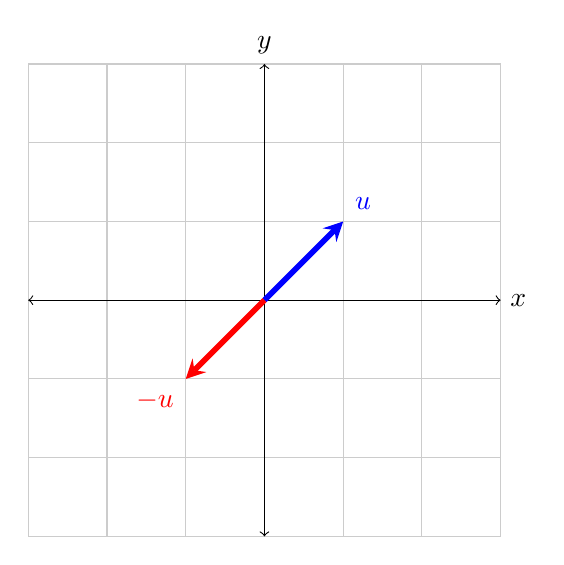
\begin{tikzpicture}
	\draw[thin,gray!40] (-3,-3) grid (3,3);
	\draw[<->] (-3,0)--(3,0) node[right]{$x$};
	\draw[<->] (0,-3)--(0,3) node[above]{$y$};
	\draw[line width=2pt,blue,-stealth](0,0)--(1,1) node[anchor=south west]{$\boldsymbol{u}$};
	\draw[line width=2pt,red,-stealth](0,0)--(-1,-1) node[anchor=north east]{$\boldsymbol{-u}$};
\end{tikzpicture}

\printbibliography[heading=subbibliography]
\end{refsection}
